\section{Offline template generation using 3D meshes and OpenGL}
In order to efficiently train the object database for each model, it is needed
to create a big set of templates, which is able to cover the whole set of view
points. Training can be performed with either \emph{online} methods (i.e.
Physically looking at the object from different viewpoints with the chosen
camera) or \emph{offline} ones, which build the dataset starting from known
object informations such as pre-extracted colour features or shape informations.

In this section we present the proposed method for template database
creation, which is an implementation of the method used by modern template
matching algorithms such as \cite{linemod-paper} and \cite{TODO}, and
has the advantage of being quite fast, fully automated for any dataset size,
and highly scalable (different datasets from different vendors can be merged
together or distributed with no effort at all).

\subsection{Offline training advantages}
It has been suggested in \cite{TODO} that fully-automated, offline training method can
outperform online training methods used as a de-facto standard
in previous years \cite{TODO}. Main advantages of offline training methods like
the proposed one, with respect
to online ones, include:

\begin{itemize}
  \item{Offline training does not require human intervention. Human-based
      training is error prone, and cannot yield to good results if not done by an
      \emph{expert} person. In an industrial or research scenario, this implies
      employing a skilled human resource in a non-productive task, which has obvious
      consequences in terms of costs (at least if the process is repeated
      for a big group of objects) and team productivity (the charged person will be
      actually involved full-time in a task which is well below is actual
    capabilities);}
  \item{Accurate training is a time-consuming task and physical objects must be available. In an
      industrial scenario, this can mean a longer time-to-market or delayed custom products deli-
      very. On the other hand, offline training does not require a physical copy of the object: for
      example, the proposed approach only needs a CAD model of the object, which in modern
      scenarios is available well before the final product; this means that training can be done at
      early project phases, before the objects used for testing the project actually
    arrive;}
  \item{If offline training is accurate enough, it can bring much more precise results than online
      one. For example, pose information associated with each template are exact when generated
    offline, while naturally subject to human error if estimated online;}
  \item{Large objects can be modelled without the need of physical movement around them. As
      algorithms such as \cite{linemod-pipeline} will probably evolve their already good real-time capabilities, they will
      be able to be applied to environments such as cities, in which the traceable objects are too
    big to be modelled online at low cost.}
\end{itemize}

\subsection{CAD modelling of objects} \label{sec:cad-mesh}
The idea behind the training procedure is to exploit CAD models of the object
to recognize in order to generate realistic renders of it and use the latter
for feature extraction and database training. In this way, a physical camera is
simulated and full viewpoints' coverage can be easily obtained.

For the purpose of the thesis, meshes have been built with Blender
\footnote{www.blender.org} and FreeCAD \footnote{www.freecad.org}. The first is a
well-established free (GPL) software for 3D graphics, while the second is an
emerging free (LGPL) general-purpose CAD application. After modelling each
object with the CAD capabilities of FreeCAD, the corresponding mesh has been
exported using a common file interchange format (\texttt{.obj}) and has been
textured in blender by using photos of the object taken with a digital camera,
exploiting Blender's advanced UV unwrapping and mapping capabilities. The result
is a realistic model of the object like the one shown in fig.
\ref{fig:realistic_rendering}, correctly textured to mimic the real one.

\begin{figure}[htbp] \label{fig:realistic_rendering}
\centering
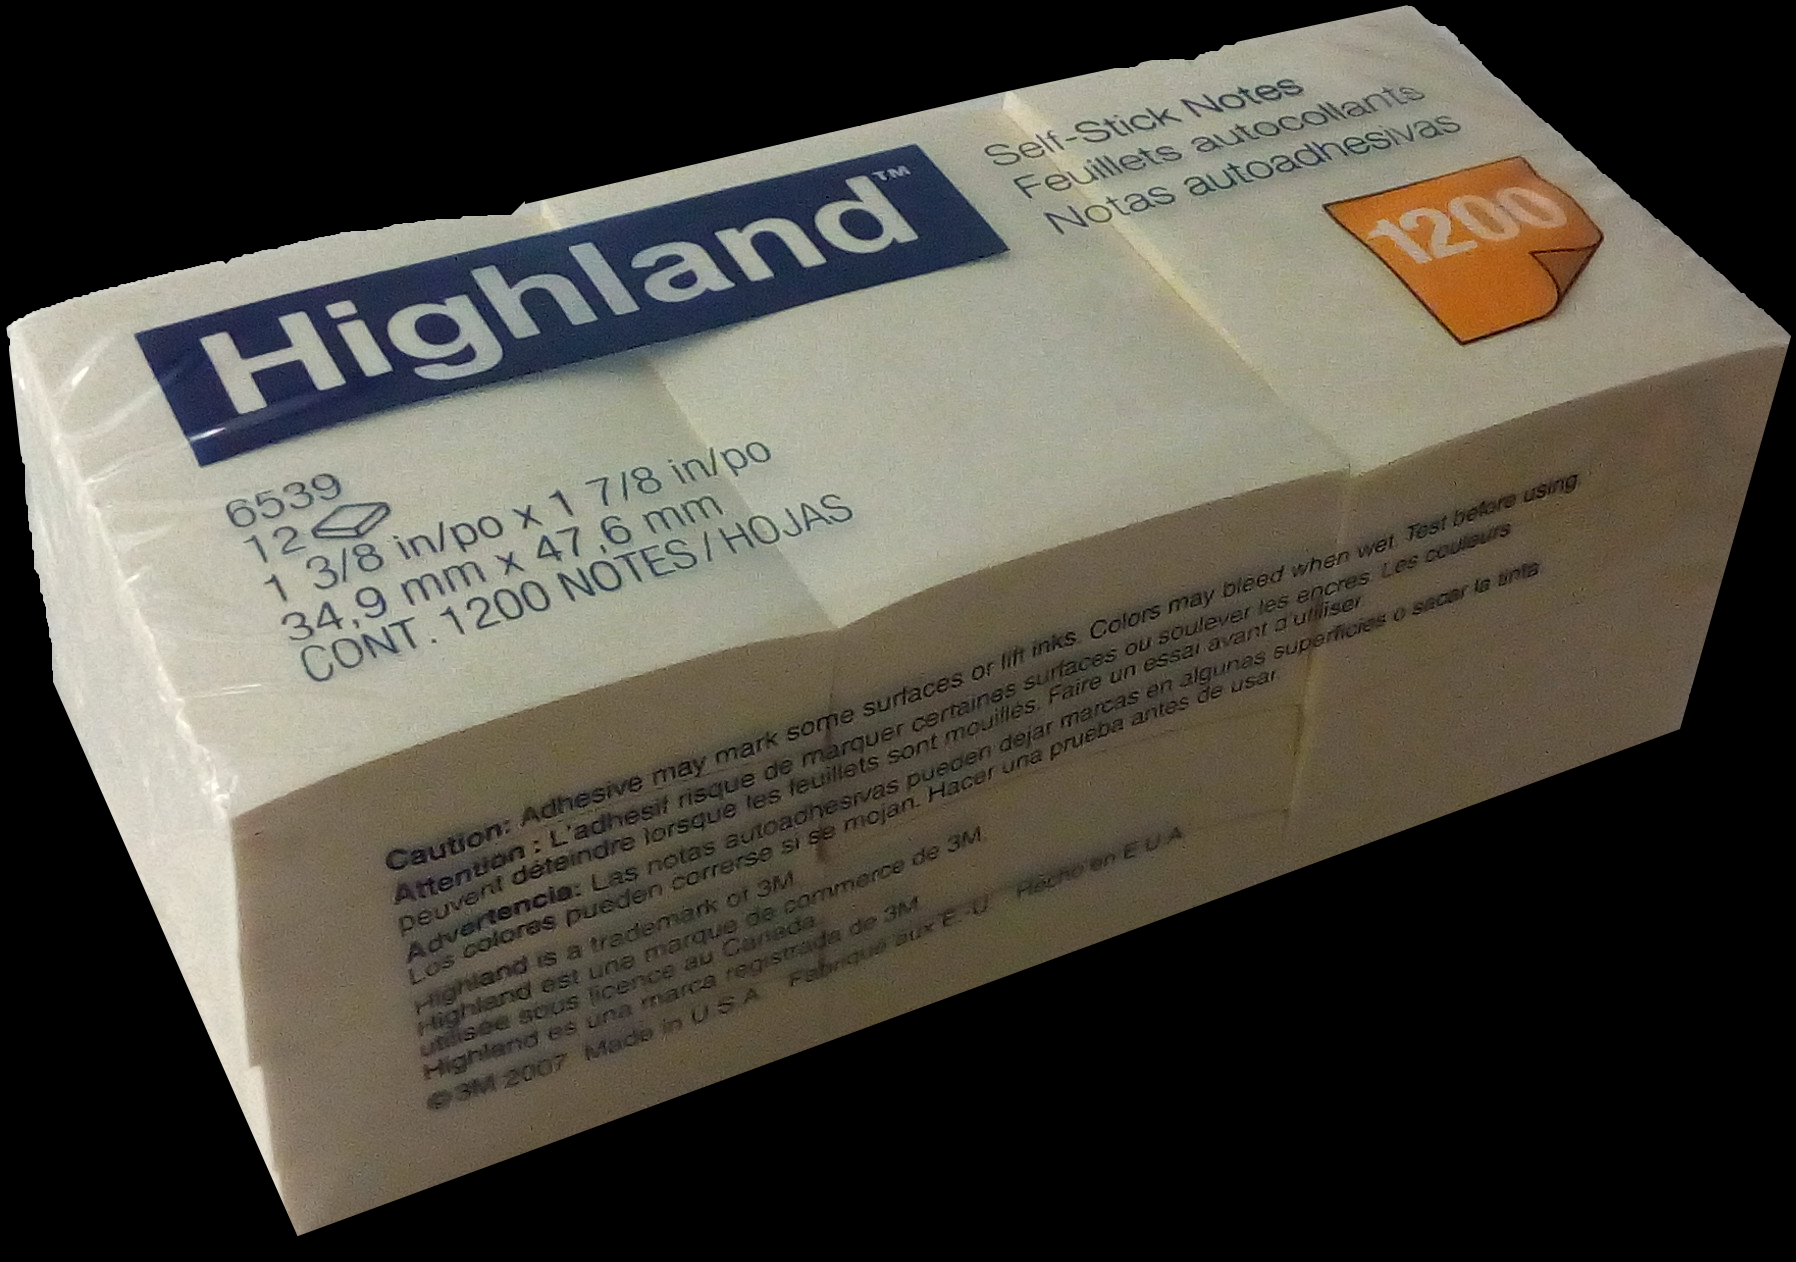
\includegraphics[height=1.5in]{./Results/postit_photo}

\includegraphics[height=1.5in]{./Results/postit_render}
\caption{Example rendering of mesh: the rendered mesh (right) is photo realistic
  if compared to real images (left),
and thus adequate to be used for template generation.}
\end{figure}

\subsection{Enumeration of possible object's positions}
The problem of covering the whole viewpoints' set for a particular object
implies a tight compromise between training speed, execution speed and
reliability. In fact, the number of templates needed for a particular object increases
both training time and recognition time. However, as the training procedure is
fully automated and not very long (about 15 minutes per object, as depicted in sec.
\ref{sec:results-time}), %TODO results-time cite check
the running time of the recognition algorithm is the main problem if too much
templates are generated. On the other side, if the object is not trained enough
at different positions and values, it could be not recognized correctly and the
whole algorithm could then fail.

The first discriminant to ensure running time is not wasted is not having
redundancy when enumerating possible poses: this excludes enumerating them via
increasing Euler Angles, as they can generate redundant transformations.

The chosen solution is to virtually keep the object still in the origin and
moving the camera around it, on the surface of a sphere of increasing radius.
This allows to enumerate all the rotations once, and at different distances too.

Two main methods exist to generate points on a sphere, which are the same
used by mainstream 3D graphics tools for mesh generation: U-V coordinates (i.e.
increasing latitudes and longitudes), and icosahedron cutting (the result of
which is called \emph{icosphere}). 

As depicted in fig. \ref{fig:uvsphere_vs_icosphere}, generating a sphere by changing latitude and longitudes of points has the 
disadvantage of having different points' densities between the poles and at the
equator, as changing longitudes results in a smaller movement if latitude is
near poles. 

The second -- and chosen -- method consists of starting approximating the sphere
as a convex icosahedron, and then iteratively subdividing each face in four
smaller faces, keeping the same radius in order to better approximate the sphere
itself. It can be easily seen that this is the best method to provide uniform
sampling method on the whole surface of the sphere, as each point will always be
at the same distance from its neighbours. 

\begin{figure}[htbp] \label{fig:uvsphere_vs_icosphere}
\centering
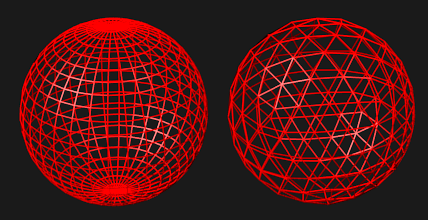
\includegraphics[width=4in]{./Graphics/uvsphere_vs_icosphere}
\caption{UV sphere (left) and icosphere (right): the latter has uniform distance
between points, which is a desirable property.}
\end{figure}

After subdividing the sphere and reaching the minimum required number of points,
the camera is moved onto each point and rotated in-plane, in order to complete
the enumeration of poses. The whole process is repeated at small distance steps
(5\~10\unit{cm}), so that the object can be recognized at different positions too.

After generating camera's position, its rotation is generated by computing the
camera's $\vec{up}$ vector (as defined by OpenGL \cite{opengl-book}) as a linear
combination of the vector perpendicular to the point's vector, heading to the
north pole, and the vector perpendicular to the point's vector, with horizontal
direction, heading east:

\begin{equation}
  \begin{array}{ccc}
  \vec{h} & = & \frac{ p  \times \vec{Z}}{\left\lVert p  \times \vec{Z}
  \right\rVert} \\
  \vec{v} & = & \frac{ p  \times \vec{Y}}{\left\lVert p  \times \vec{Y}
  \right\rVert} \\
  \alpha_i & = & \frac{2\pi}{i_{max}} i \\
  \vec{up}_i & = & \vec{h} \sin(\alpha_i) + \vec{v} \cos (\alpha_i)
  \end{array}
\end{equation}

Knowing camera's position $\vec{P_c}$ and $\vec{up}$ vector, the transformation matrix of
the camera with respect to origin can be computed as done in OpenGL:

\begin{equation}
  \begin{array}{ccc}
  \vec{f} & = & -\vec{P_c} \\
  \vec{s} & = & \vec{f} \times \vec{up} \\ 
  \vec{u} & = & \left( \frac{\vec{s} }{\left\lVert \vec{s}\right\rVert} 
  \right) \times \vec{f} \\
  M & = & \left(
  \begin{array}{cc}
    s & -x_c \\
    u & -y_c \\
    -f & -z_c  \\
    \vec{0} & 1
  \end{array} 
  \right) \\
  \end{array}
\end{equation}

\begin{figure}[htbp] \label{fig:up_vector}
\centering
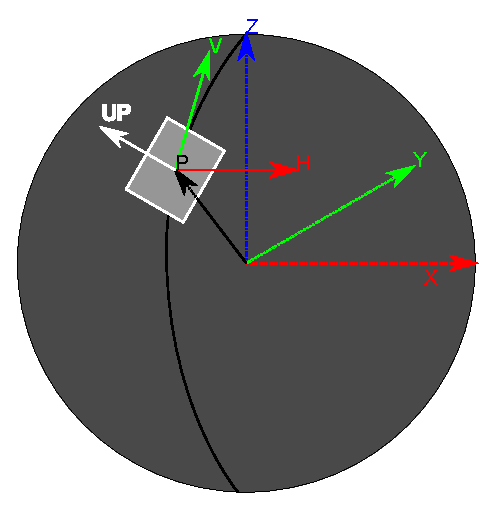
\includegraphics[width=3in]{./Graphics/up_vector}
\caption{In-plane rotation of camera by generating $\vec{up}$ vector as a linear
combination of plane's direction vectors}
\end{figure}

This matrix is finally inverted to transform it in the object's position
relative to the camera, as it is in the coordinate system of the latter that the
object's pose will be estimated.

The object is then rendered on RGBD images into its position using the OpenGL renderer
described in sec. \ref{sec:opengl-rendering}. The rendered RGBD image, together
with the object's mask generated from rendering, is finally passed to the chosen
detector in order to extract a template.
